We are interested in the dynamics that emerge when fixing the parameters $\beta = 1, f = 150, L = 4.2 \cdot 10^{-3}, R = 2, V_m = 5,$ and $\mu = 0.5$.
The parameters $E_0$ and $\chi_0$ are varied.
$E_0$ is in the range $[14, 28]$, while $\chi_0$ is in the range $[0.1, 0.65]$.
When scanning this parameter plane for the period of emerging cycles, \Cref{fig:yunus.2pi.2d.full} emerges.

\begin{figure}
    \centering
    \includegraphics[width=0.6\textwidth]{99_Yunus/2D_Period/result.png}
    \caption{2D Scan of Original Model}
    \label{fig:yunus.2pi.2d.full}
\end{figure}

The thing, we are interested in, is what happens along the red line.
The period stays the same, but the area, where this period is, gets thinner at this point.
\Cref{fig:yunus.2pi.CobwebA2,fig:yunus.2pi.CobwebB2} show what happens right at the beginning of the thin area.
When you follow the blue line in \Cref{fig:yunus.2pi.CobwebB2}, you see that there are two cycles of period 12 coexisting.
In \Cref{fig:yunus.2pi.CobwebA2} there was only one cycle of period 12.
Its symbolic sequence is $\A^3\B^3\C^3\D^3$.
This cycle disappears at the beginning of the thin area and two new cycles of period 12 emerge.
You can see the in \Cref{fig:yunus.2pi.CobwebB2}.
Their symbolic sequences are $\A^3\B^3\C^2\D^4$ and $\A^2\B^4\C^3\D^3$ respectively.

\Cref{fig:yunus.2pi.CobwebC2,fig:yunus.2pi.CobwebD2} show what happens right at the end of the thin area.
In \Cref{fig:yunus.2pi.CobwebC2} there are still the two coexisting cycles described above.
But in \Cref{fig:yunus.2pi.CobwebD2}, they both disappear and a new cycle emerges.
Its symbolic sequence is $\A^2\B^4\C^2\D^4$.

\begin{figure}
    \centering
    \begin{subfigure}{0.4\textwidth}
        \centering
        \includegraphics[width=\textwidth]{99_Yunus/Period12/Cobweb_A2/result.png}
        \caption{Before the thin area begins}
        \label{fig:yunus.2pi.CobwebA2}
    \end{subfigure}
    \begin{subfigure}{0.4\textwidth}
        \centering
        \includegraphics[width=\textwidth]{99_Yunus/Period12/Cobweb_B2/result.png}
        \caption{After the thin area begins}
        \label{fig:yunus.2pi.CobwebB2}
    \end{subfigure}
    \begin{subfigure}{0.4\textwidth}
        \centering
        \includegraphics[width=\textwidth]{99_Yunus/Period12/Cobweb_C2/result.png}
        \caption{Before the thin area ends}
        \label{fig:yunus.2pi.CobwebC2}
    \end{subfigure}
    \begin{subfigure}{0.4\textwidth}
        \centering
        \includegraphics[width=\textwidth]{99_Yunus/Period12/Cobweb_D2/result.png}
        \caption{After the thin area ends}
        \label{fig:yunus.2pi.CobwebD2}
    \end{subfigure}
    \caption{Cobwebs of Full Original Model}
\end{figure}
